\section{Illustration of the system}
The reason for making a rich picture is to help one understand the interaction within a specific technology and/or product. The picture in \vref{fig:Rig billede} is an overview of how the administrators (parents and kindergarten teachers) and the child would interact with the mobile device. Under the assumption that the multi-bachelor project \textit{GIRAF} has been implemented in everyday life, we want to show how it could be improved with an administrator program on the computer.

In the current system, the person responsible for administrating the settings, programs and data on the mobile device, has to accomplish that on the mobile device itself. At the same time the child may also have need for the mobile device, creating conflict between child and administrator when the mobile device is needed at both sides at the same time. The mobile device is used by the child as a communication tool so the administrators are able to understand what the child wants or needs. 
Though this understanding the child and administrator can easier communicate in their everyday life.%?WTF?

The problem with the current \textit{GIRAF} system is that both the administrator and child need the same mobile device. Some children will consider the mobile device theirs and therefore will not hand it over to the administrator or do so with much frustration. To resolve this problem, a computer program could be made, from where the administrator could administer the mobile device's settings and data via some form of a wireless connection. This picture is shown in \vref{fig:Rig billede}. 

\begin{figure}[ht]
	\centering
		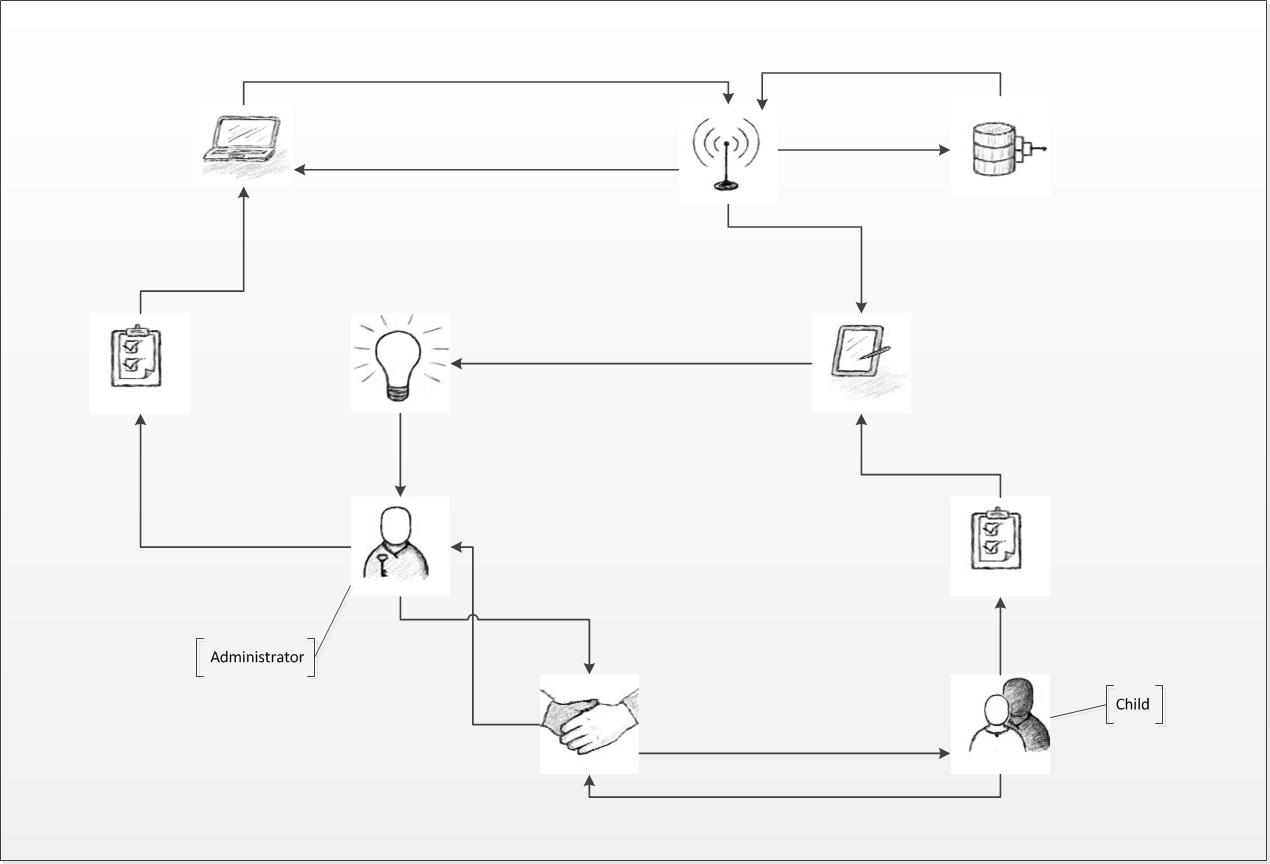
\includegraphics[width=1.00\textwidth]{img/Rig_billede.jpg}
	\caption{How the solutions should be}
	\label{fig:Rig billede}
\end{figure}

In our project we also want to make a digitized version of the contact book so that kindergarten teachers and parents, easily and quickly, can exchange information. Furthermore the kindergarten teachers would then be able to write and send a summary of the child's activities including pictures of the involved activites. This is the base for our system definition.    